
Cho một sợi dây thép cứng, nhẵn được uốn thành đa giác lồi $N$ cạnh có chiều dài các cạnh là $l_1, l_2,..., l_N$ và mặt bàn nhẵn nằm ngang có hình dạng giống hệt đa giác ở trên.
\begin{enumerate}[label=(\alph*)]
\item Ta uốn sợi dây thành đa giác đều ($l_1=l_2=...=l_N=l$). Giả sử rằng ta có $N$ ròng rọc rất nhỏ và rất nhẹ luồn vào từng cạnh của đa giác, sau đó buộc $N$ sợi dây nhẹ, không dãn sao cho một đầu được nối vào quả nặng $M$, đầu còn lại được nối vào những khối lượng bằng nhau có khối lượng $m$. Đặt khối lượng $M$ lên bàn và vắt mỗi sợi dây lên các ròng rọc có chỉ số các cạnh tương ứng (như hình vẽ bên dưới). Xét trong vùng mà mỗi cạnh của đa giác chỉ chứa một ròng rọc, hãy xác định các vị trí cân bằng trong khu vực này. Vẽ hình chỉ ra vị trí cân bằng cho trường hợp $N=5$ và $N=6$.

\begin{figure}[!h]
    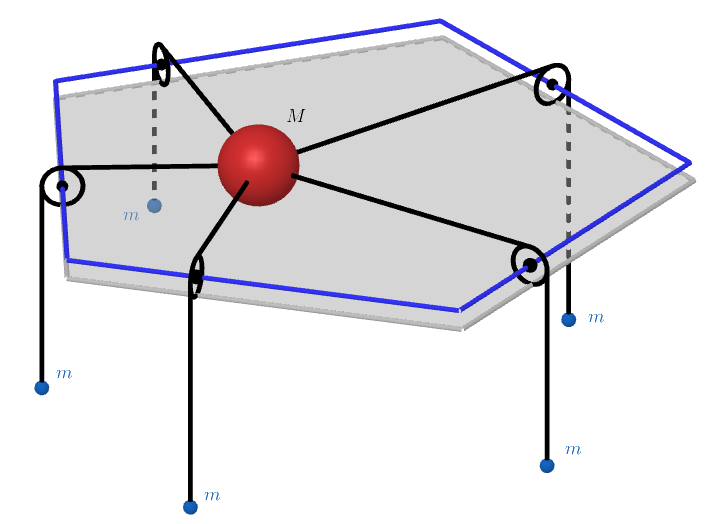
\includegraphics[width=0.5\linewidth]{Problem_1/Figs_P1/Figs_P1.png}
    \centering
    \label{fig:P1_01}
    \caption{}
\end{figure}
\item Xét trường hợp $N = 3$ (nói cách khác là cuốn sợi dây thành hình tam giác có cạnh $l_1, l_2, l_3$), sau đó luồn 3 hạt cườm rất nhẹ vào mỗi cạnh, mỗi hạt cườm lại có một lò xo có độ dài tự nhiên rất nhỏ (coi bằng 0) có độ cứng $k_1, k_2, k_3$ và một đầu của mỗi lò xo được gắn vào khối lượng $M$ (như hình ở dưới). Đặt vật $M$ trên bàn. Xác định vị trí cân bằng trong các trường hợp:
    \begin{enumerate}[label=(\roman*)]
    \item Độ dài các cạnh của tam giác và các độ cứng của lò xo thỏa mãn: $l_1:l_2:l_3=k_1:k_2:k_3$.
    \item Các độ cứng của lò xo bằng nhau và bằng $k$.
    \end{enumerate}
\begin{figure}[H]
    \centering
    % Gradient Info
  
\tikzset {_2c9ddldf2/.code = {\pgfsetadditionalshadetransform{ \pgftransformshift{\pgfpoint{89.1 bp } { -128.7 bp }  }  \pgftransformscale{1.32 }  }}}
\pgfdeclareradialshading{_8o830cp2v}{\pgfpoint{-72bp}{104bp}}{rgb(0bp)=(0.89,0.75,0.75);
rgb(0bp)=(0.89,0.75,0.75);
rgb(12.589285714285714bp)=(0.82,0.01,0.11);
rgb(400bp)=(0.82,0.01,0.11)}
\tikzset{every picture/.style={line width=0.75pt}} %set default line width to 0.75pt        

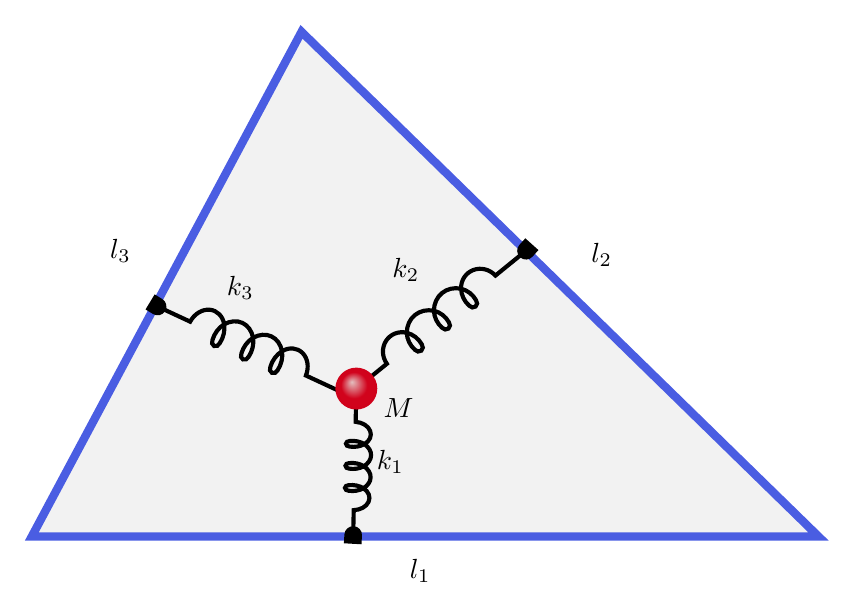
\begin{tikzpicture}[x=0.75pt,y=0.75pt,yscale=-1,xscale=1]
%uncomment if require: \path (0,462); %set diagram left start at 0, and has height of 462

%Shape: Triangle [id:dp3326541587702424] 
\draw  [color={rgb, 255:red, 74; green, 93; blue, 226 }  ,draw opacity=1 ][fill={rgb, 255:red, 128; green, 128; blue, 128 }  ,fill opacity=0.1 ][line width=3]  (179.94,26) -- (429,269.11) -- (50,269.11) -- cycle ;
%Shape: Inductor (Air Core) [id:dp6872930774599556] 
\draw  [line width=1.5]  (206.28,201.94) -- (206.02,213.91) .. controls (209.3,214.15) and (212.07,215.88) .. (213,218.25) .. controls (213.93,220.62) and (212.83,223.16) .. (210.23,224.64) .. controls (208.2,225.79) and (205.6,226.21) .. (203.09,225.82) .. controls (202.11,225.8) and (201.33,225.18) .. (201.35,224.45) .. controls (201.36,223.71) and (202.17,223.14) .. (203.15,223.16) .. controls (205.67,222.87) and (208.25,223.41) .. (210.23,224.64) .. controls (212.33,226.07) and (213.5,228.02) .. (213.45,230.03) .. controls (213.41,232.05) and (212.16,233.94) .. (209.99,235.28) .. controls (207.97,236.42) and (205.37,236.85) .. (202.86,236.45) .. controls (201.88,236.43) and (201.1,235.82) .. (201.12,235.08) .. controls (201.13,234.35) and (201.94,233.77) .. (202.92,233.79) .. controls (205.44,233.51) and (208.02,234.05) .. (209.99,235.28) .. controls (212.1,236.71) and (213.26,238.66) .. (213.22,240.67) .. controls (213.18,242.68) and (211.93,244.58) .. (209.76,245.91) .. controls (207.73,247.06) and (205.14,247.49) .. (202.63,247.09) .. controls (201.65,247.07) and (200.87,246.45) .. (200.88,245.72) .. controls (200.9,244.99) and (201.71,244.41) .. (202.69,244.43) .. controls (205.21,244.14) and (207.79,244.68) .. (209.76,245.91) .. controls (212.3,247.51) and (213.28,250.09) .. (212.25,252.42) .. controls (211.22,254.75) and (208.38,256.35) .. (205.09,256.45) -- (204.83,268.42) ;
%Shape: Inductor (Air Core) [id:dp16634280228018206] 
\draw  [line width=1.5]  (110.6,158.34) -- (126.29,165.64) .. controls (128.31,161.89) and (132.02,159.61) .. (135.64,159.89) .. controls (139.25,160.17) and (142.04,162.96) .. (142.66,166.91) .. controls (143.12,169.99) and (142.34,173.32) .. (140.52,176.06) .. controls (139.99,177.21) and (138.77,177.79) .. (137.81,177.34) .. controls (136.85,176.89) and (136.5,175.59) .. (137.04,174.44) .. controls (137.96,171.28) and (140.01,168.54) .. (142.66,166.91) .. controls (145.63,165.25) and (148.82,165.01) .. (151.46,166.23) .. controls (154.09,167.46) and (155.96,170.05) .. (156.6,173.4) .. controls (157.06,176.48) and (156.29,179.81) .. (154.46,182.55) .. controls (153.93,183.7) and (152.71,184.27) .. (151.75,183.83) .. controls (150.79,183.38) and (150.44,182.08) .. (150.98,180.93) .. controls (151.9,177.77) and (153.95,175.03) .. (156.6,173.4) .. controls (159.58,171.74) and (162.76,171.49) .. (165.4,172.72) .. controls (168.04,173.95) and (169.9,176.54) .. (170.54,179.89) .. controls (171.01,182.96) and (170.23,186.3) .. (168.41,189.04) .. controls (167.87,190.19) and (166.66,190.76) .. (165.69,190.31) .. controls (164.73,189.86) and (164.39,188.57) .. (164.92,187.42) .. controls (165.85,184.26) and (167.89,181.51) .. (170.54,179.89) .. controls (173.97,177.81) and (177.89,178.15) .. (180.44,180.74) .. controls (182.98,183.32) and (183.63,187.63) .. (182.06,191.59) -- (197.75,198.88) ;
%Shape: Inductor (Air Core) [id:dp3092264128133372] 
\draw  [line width=1.5]  (206.35,197.88) -- (221.06,185.93) .. controls (218.69,182.58) and (218.53,178.21) .. (220.65,174.91) .. controls (222.77,171.61) and (226.73,170.06) .. (230.65,171.01) .. controls (233.68,171.76) and (236.31,173.78) .. (237.87,176.55) .. controls (238.64,177.5) and (238.53,178.86) .. (237.63,179.6) .. controls (236.72,180.33) and (235.37,180.16) .. (234.6,179.21) .. controls (232.2,177.12) and (230.76,174.13) .. (230.65,171.01) .. controls (230.67,167.56) and (232.08,164.47) .. (234.56,162.46) .. controls (237.03,160.45) and (240.35,159.7) .. (243.72,160.38) .. controls (246.76,161.13) and (249.39,163.15) .. (250.94,165.93) .. controls (251.71,166.88) and (251.61,168.24) .. (250.7,168.97) .. controls (249.8,169.71) and (248.44,169.53) .. (247.67,168.58) .. controls (245.28,166.49) and (243.84,163.5) .. (243.72,160.38) .. controls (243.75,156.94) and (245.16,153.85) .. (247.64,151.84) .. controls (250.11,149.82) and (253.43,149.07) .. (256.8,149.76) .. controls (259.84,150.51) and (262.47,152.53) .. (264.02,155.3) .. controls (264.79,156.25) and (264.68,157.62) .. (263.78,158.35) .. controls (262.88,159.08) and (261.52,158.91) .. (260.75,157.96) .. controls (258.36,155.87) and (256.92,152.88) .. (256.8,149.76) .. controls (256.68,145.73) and (259.01,142.17) .. (262.67,140.77) .. controls (266.33,139.37) and (270.58,140.42) .. (273.37,143.43) -- (288.08,131.48) ;
%Flowchart: Delay [id:dp8143670880210933] 
\draw  [fill={rgb, 255:red, 0; green, 0; blue, 0 }  ,fill opacity=1 ] (109.35,153.2) -- (112.55,155.15) .. controls (114.31,156.22) and (114.87,158.52) .. (113.8,160.28) .. controls (112.73,162.05) and (110.43,162.61) .. (108.66,161.54) -- (105.47,159.59) -- cycle ;
%Flowchart: Delay [id:dp9198941962672681] 
\draw  [fill={rgb, 255:red, 0; green, 0; blue, 0 }  ,fill opacity=1 ] (200.88,271.94) -- (201.1,268.2) .. controls (201.22,266.14) and (202.99,264.57) .. (205.05,264.69) .. controls (207.11,264.81) and (208.68,266.58) .. (208.56,268.64) -- (208.35,272.37) -- cycle ;
%Flowchart: Delay [id:dp3222573149762976] 
\draw  [fill={rgb, 255:red, 0; green, 0; blue, 0 }  ,fill opacity=1 ] (293.37,131.19) -- (290.87,133.97) .. controls (289.49,135.51) and (287.12,135.64) .. (285.59,134.26) .. controls (284.05,132.88) and (283.92,130.51) .. (285.3,128.98) -- (287.8,126.19) -- cycle ;
%Flowchart: Connector [id:dp4674995309000146] 
\path  [shading=_8o830cp2v,_2c9ddldf2] (196.75,197.88) .. controls (196.75,192.58) and (201.05,188.29) .. (206.35,188.29) .. controls (211.64,188.29) and (215.94,192.58) .. (215.94,197.88) .. controls (215.94,203.18) and (211.64,207.47) .. (206.35,207.47) .. controls (201.05,207.47) and (196.75,203.18) .. (196.75,197.88) -- cycle ; % for fading 
 \draw  [color={rgb, 255:red, 208; green, 2; blue, 27 }  ,draw opacity=1 ][line width=0.75]  (196.75,197.88) .. controls (196.75,192.58) and (201.05,188.29) .. (206.35,188.29) .. controls (211.64,188.29) and (215.94,192.58) .. (215.94,197.88) .. controls (215.94,203.18) and (211.64,207.47) .. (206.35,207.47) .. controls (201.05,207.47) and (196.75,203.18) .. (196.75,197.88) -- cycle ; % for border 


% Text Node
\draw (230.7,278.69) node [anchor=north west][inner sep=0.75pt]    {$l_{1}$};
% Text Node
\draw (318.07,126.28) node [anchor=north west][inner sep=0.75pt]    {$l_{2}$};
% Text Node
\draw (86.23,124.46) node [anchor=north west][inner sep=0.75pt]    {$l_{3}$};
% Text Node
\draw (214.79,226.02) node [anchor=north west][inner sep=0.75pt]    {$k_{1}$};
% Text Node
\draw (222.27,133.76) node [anchor=north west][inner sep=0.75pt]    {$k_{2}$};
% Text Node
\draw (142.48,142.07) node [anchor=north west][inner sep=0.75pt]    {$k_{3}$};
% Text Node
\draw (217.94,201.28) node [anchor=north west][inner sep=0.75pt]    {$M$};
\end{tikzpicture}
\centering
\caption{}
\label{fig:P1_02}
\end{figure}
\end{enumerate}

Gợi ý: Có thể sử dụng định lý con nhím cho đa giác $N$ cạnh, tức là: 
\begin{equation}
l_1\vec{\hat{n}_1}+l_2\vec{\hat{n}_2}+...+l_N\vec{\hat{n}_N}=\vec{0}.
\end{equation}
Trong đó $\vec{\hat{n}_i}$ là vector đơn vị pháp tuyến với cạnh thứ $i$, hướng ra ngoài đa giác.

Hoặc có thể sử dụng việc vật đạt trạng thái cân bằng (bền) thì thế năng sẽ đạt giá trị cực tiểu.